% +++
% sequence = ["latex", "bibtex", "latex", "latex"]
% [programs.latex]
% 	command = "lualatex"
% 	opts = ["-synctex=1", "-file-line-error", "-interaction=nonstopmode"]
% 	args = ["%S"]
% [programs.bibtex]
% 	command = "upbibtex"
% 	target = "../ref.bib"
% 	args = ["%B"]
% +++

\documentclass[../main/thesis_template]{subfiles}
\graphicspath{{\subfix{../contents/figures/section2/}}}
\setcounter{section}{1}

\begin{document}
\section{次のSection}
\addtocontents{lof}{\protect\addvspace{1em}}

\subsection{Boltzmann方程式}
希薄気体の支配方程式はBoltzmann方程式と呼ばれ, 外力がない場合には次のように表される.
\begin{align}
  \frac{\partial f}{\partial t} &+ \bm{\xi}\cdot\frac{\partial f}{\partial \bm{x}}=J[f], 
    \label{eq:Boltzmann}\\
  J[f] 
    &= \int_{|\bm{\xi}|<\infty,|\bm{\alpha}|=1}
      \left[ f(\bm{\xi^\prime})f(\bm{\zeta^\prime})-f(\bm{\xi})f(\bm{\zeta}) \right] 
      \left( \frac{d_m^2}{2}|\bm{V}\cdot\bm{\alpha}|\right)
      \diff\Omega(\bm{\alpha})\diff\bm{\zeta}, \notag\\
  \bm{V} &= \bm{\zeta} - \bm{\xi}, \qquad
  \bm{\xi^\prime} = \bm{\xi} + \left(\bm{V}\cdot\bm{\alpha}\right)\bm{\alpha}, \qquad
  \bm{\zeta^\prime} = \bm{\zeta} + (\bm{V}\cdot\bm{\alpha})\bm{\alpha}. \notag
\end{align}
ここで, $\bm{x}$は空間3次元の位置座標, $\bm{\xi}$は気体分子の速度ベクトル, $t$は時刻, $f(\bm{x},\bm{\xi},t)$は速度分布関数, $J[f]$は衝突項である.
また, $\partial f/\partial\bm{x}=(\partial f/\partial x,\partial f/\partial y,\partial f/\partial z)^\top$を表すものとする.
ここで${}^\top$は転置を表す.
$d_m$は気体分子の直径, $\bm{\alpha}$は分子の衝突パラメータ, $\diff\Omega(\bm{\alpha})$は立体角素である.
気体の巨視的物理量は速度分布関数$f(\bm{x},\bm{\xi},t)$に関する積分によって表される.
気体の数密度$n$, 流速$\bm{v}$, 温度$T$, 応力テンソル$p_{ij}$はそれぞれ
\begin{subeq}
\begin{align}
  n(\bm{x},t) &= 
    \int_{|\bm{\xi}|<\infty}
    f(\bm{x},\bm{\xi},t) \,\diff\bm{\xi}, \label{eq:n}\\
  n\bm{v}(\bm{x},t) &= 
    \int_{|\bm{\xi}|<\infty}
    \bm{\xi}f(\bm{x},\bm{\xi},t) \,\diff\bm{\xi}, \label{eq:v}\\
  \frac{3}{2} \kappa n T(\bm{x},t) &= 
    \int_{|\bm{\xi}|<\infty}
    \frac{m}{2}|\bm{\xi}-\bm{v}|^2f(\bm{x},\bm{\xi},t) \,\diff\bm{\xi}, 
    \label{eq:T}\\
  (p_{ij}+\rho v_iv_j)(\bm{x},t) &= 
    \int_{|\bm{\xi}|<\infty}
    m\,\xi_i\xi_jf(\bm{x},\bm{\xi},t)\,\diff\bm{\xi} \label{eq:pij}
\end{align}
によって得られる.
なお, $\kappa$はボルツマン定数, $m$は分子の質量, $\rho=mn$は気体の密度である.
今後, 気体は単原子分子の理想気体とする\cite{Asakura2022}と, 気体の圧力 $p$ は
\begin{equation}
  p = \kappa nT \label{eq:p}
\end{equation}
となる.
\end{subeq}

\begin{figure}[b]
  \centering
  \begin{subfigure}{0.65\hsize}
    \centering
    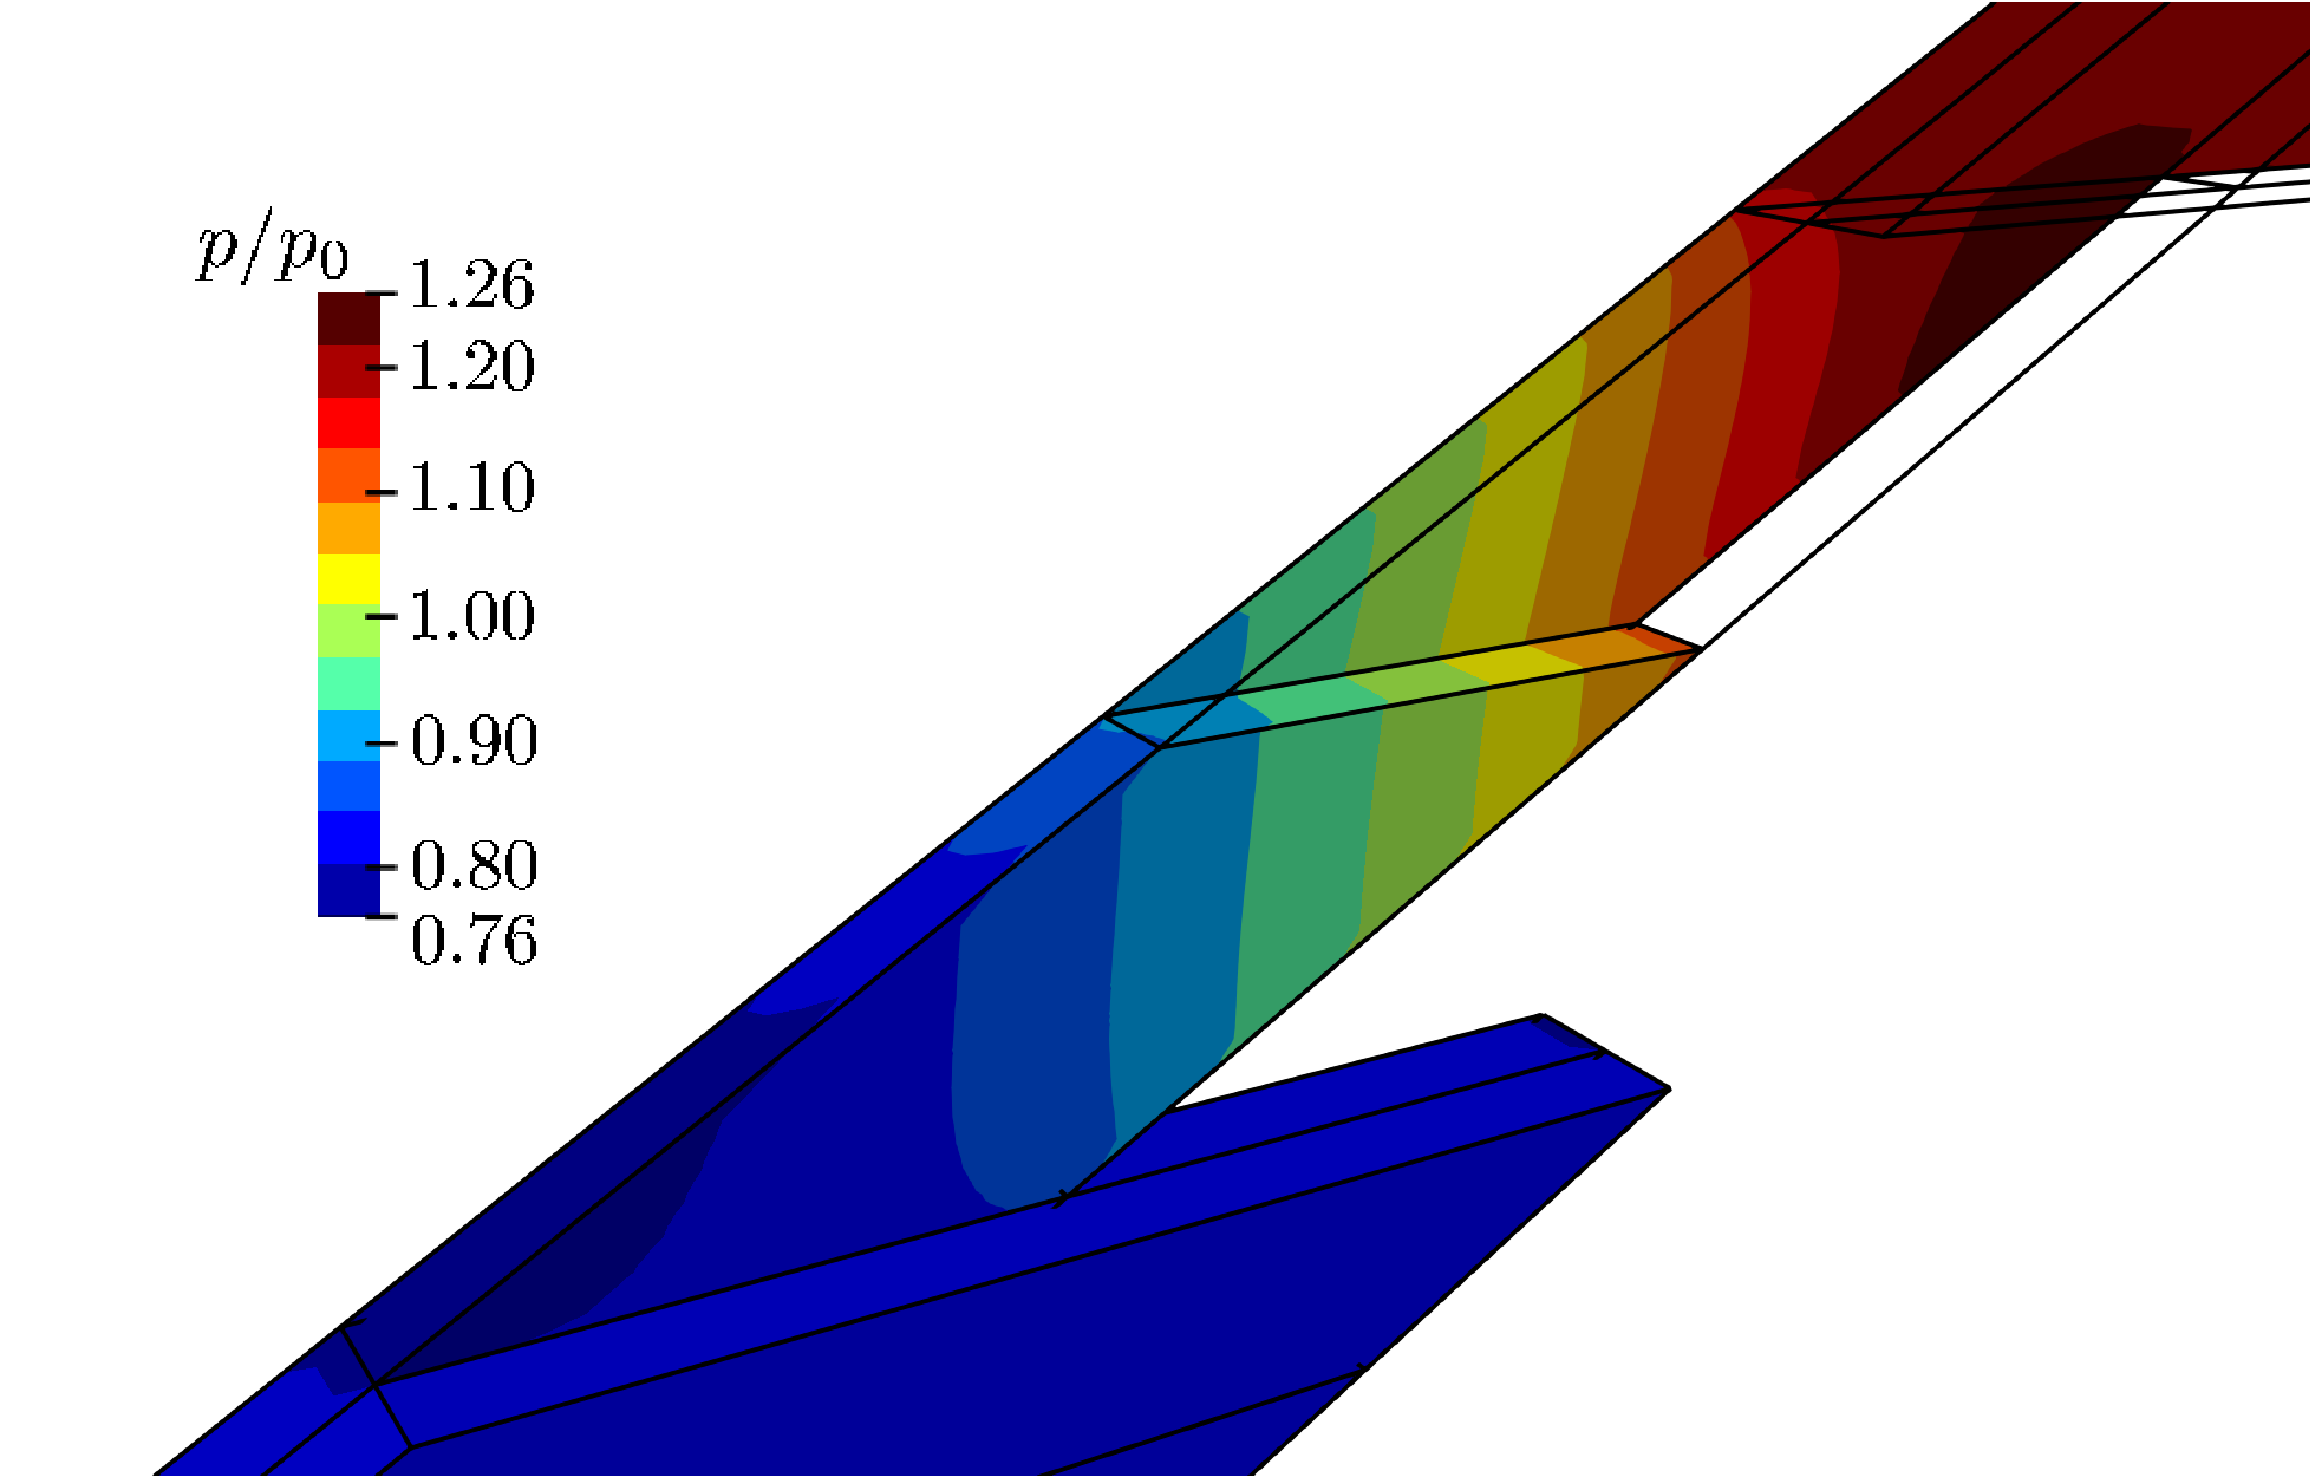
\includegraphics[width=0.9\hsize]{fig_2-1a.pdf}
    \captionsetup{skip=0em}
    \subcaption{}
    \label{fig:Inf_t-Q_Arg}
  \end{subfigure}
  \begin{subfigure}{0.3\hsize}
    \centering
    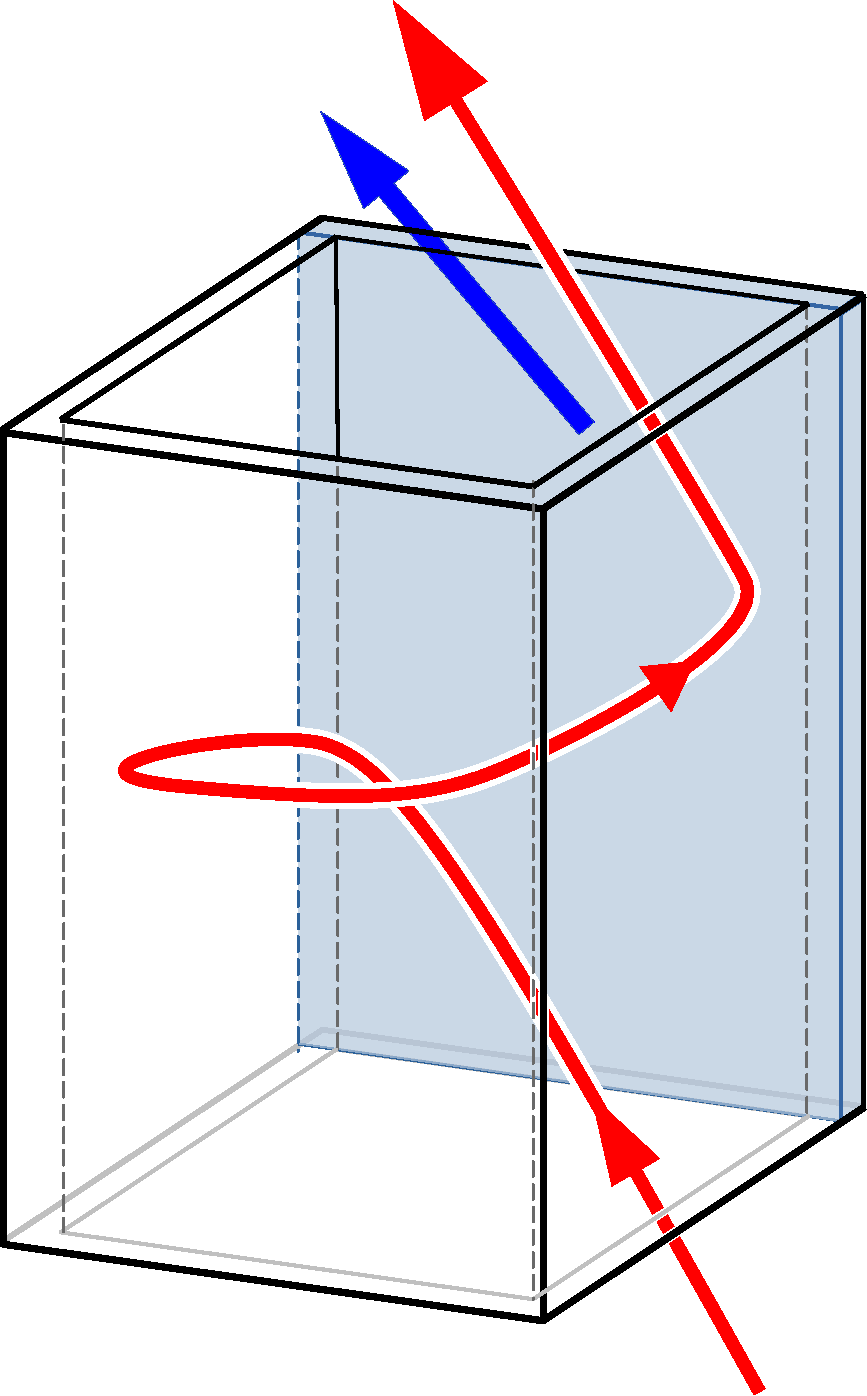
\includegraphics[width=0.9\hsize]{fig_2-1b.pdf}
    \captionsetup{skip=0em}
    \subcaption{}
    \label{fig:Inf_Arg-Q}
  \end{subfigure}
  \captionsetup{skip=-2pt}
  \caption[short caption.]{
    \begin{minipage}[t]{13em}
      short caption.\\
      explanation of figures. 
    \end{minipage}  
  }
  \label{fig:2-1}
\end{figure}


\ifSubfilesClassLoaded{%
  \printbibliography
}% 

\end{document}
